\chapter{Evaluating the goodness of estimators}

\section{Relative efficiency}

It is usually possible to retrieve more than one unbiased estimator for the same target 
parameter $\theta$. But we only prefer to use the estimator with the 
\textbf{smaller variance}. That is, if $\widehat{\theta}_1$ and $\widehat{\theta}_2$ are 
unbiased estimators for the same parameter $\theta$, we said that 
$\widehat{\theta}_1$ is \textit{relatively more efficient} than $\widehat{\theta}_2$ 
if 
\[
    Var(\widehat{\theta}_1) < Var(\widehat{\theta}_2). 
\]
In fact, this can be expressed as the ratio $ Var(\widehat{\theta}_1) / Var(\widehat{\theta}_2)$
to measure the relative efficiency of these two unbiased estimators.

\begin{definition}[Relative efficiency]
    Given two unbiased estimators $\widehat{\theta}_1$ and $\widehat{\theta}_2$ for the 
    same parameter $\theta$, with variances $Var(\widehat{\theta}_1)$ and $Var(\widehat{\theta}_2)$,
    respectively. Then the efficiency of $\widehat{\theta}_1$ relative to $\widehat{\theta}_2$, 
    wrote as $\textsf{Eff}(\widehat{\theta}_1, \widehat{\theta}_2)$, is defined to be the ratio
    \begin{equation}
        \textsf{Eff}(\widehat{\theta}_1, \widehat{\theta}_2) := \frac{Var(\widehat{\theta}_2)}{Var(\widehat{\theta}_1)}.
    \end{equation}
\end{definition}

\begin{example}
    If $Y_1, Y_2, \ldots, Y_n$ denote a random sample from the uniform distribution on the 
    interval $(0, \theta)$. The two unbiased estimators for $\theta$ are 
    \[
        \widehat{\theta}_1 = 2 \ols{Y}, \quad \widehat{\theta}_2 = \left( \frac{n+1}{n}\right) Y_{(n)},
    \]
    where $Y_{(n)} = \max\{ Y_1, Y_2, \ldots, Y_n \}$. Find the efficiency of $\widehat{\theta}_1$ relative to $\widehat{\theta}_2$.
\end{example}
\begin{solution}
    Because each $Y_i \sim U(0, \theta)$, we have
    \[
        \mu = \mathbb{E}[Y_i] = \mfrac{\theta}{2}, \quad \sigma^2 = Var(Y_i) = \frac{\theta^2}{12}.
    \]
    Therefore,
    \[
        \mathbb{E}[\widehat{\theta}_1] = \mathbb{E}(2\ols{Y}) = 2 \mathbb{E}(\ols{Y}) = 2 \mu = \theta,
    \]
    and that $\widehat{\theta}_1$ is unbiased, as claimed. Further we check that 
    \[
        Var(\widehat{\theta}_1) = Var(2\ols{Y}) = 4Var(\ols{Y}) = 4 \cdot \frac{\sigma^2}{n} = \frac{\theta^2}{3n},
    \]

    The mean of this order statistic is 
    \begin{align*}
        \mathbb{E}[Y_{(n)}] = \int^\theta_0 y \cdot n \left(\frac{y}{\theta}\right)^{n-1} \left(\frac{1}{\theta}\right)\, \mathrm{d}y
        &= \frac{n}{\theta^n} \int^\theta_0 y^n \, \mathrm{d}y\\
        &= \frac{n}{\theta^n} \left[ \frac{y^{n+1}}{n+1}\right]^{y=\theta}_{y=0}\\
        &= \frac{n\theta}{n+1}.
    \end{align*}
    and it follows that 
    \[
        \mathbb{E}\left[ \frac{n+1}{n}\, Y_{(n)} \right] = \theta;
    \]
    that is, $\widehat{\theta}_2$ is also an unbiased estimator of $\theta$. Since
    \begin{align*}
        \mathbb{E}[Y^2_{(n)}] = \int^\theta_0 y^2 \cdot n \left(\frac{y}{\theta}\right)^{n-1} \left(\frac{1}{\theta}\right)\, \mathrm{d}y
        &= \frac{n}{\theta^n} \int^\theta_0 y^{n+1} \, \mathrm{d}y\\
        &= \frac{n}{\theta^n} \left[ \frac{y^{n+2}}{n+2}\right]^{y=\theta}_{y=0}\\
        &= \frac{n\theta^2}{n+2}.
    \end{align*}

    we obtain
    \begin{align*}
        Var[Y_{(n)}] = \mathbb{E}[Y^2_{(n)}] - (\mathbb{E}[Y_{(n)}])^2
        &= \frac{n\theta^2}{n+2} - \left(\frac{n\theta}{n+1}\right)^2\\
        &= \theta^2 \left[ \frac{n}{n+2} - \frac{n^2}{(n+1)^2} \right]\\
        &= \theta^2 \left[ \frac{n(n+1)^2 - n^2(n+2)}{(n+2)(n+1)^2} \right]\\
        &= \theta^2 \left[ \frac{n^3 + 2n^2 + n - n^3 - 2n^2}{(n+2)(n+1)^2} \right]\\
        &= \frac{n \theta^2}{(n+2)(n+1)^2}.
    \end{align*}
    and hence 
    \begin{align*}
        Var[\widehat{\theta}_2] &= Var\left[ \frac{n+1}{n} Y_{(n)} \right]\\
        &= \left( \frac{n+1}{n} \right)^2 Var[Y_{(n)}]\\
        &= \left( \frac{n+1}{n} \right)^2 \cdot \frac{n \theta^2}{(n+2)(n+1)^2}\\
        &= \frac{\theta^2}{n(n+2)}.
    \end{align*}
    Therefore, the efficiency of $\widehat{\theta}_1$ relative to $\widehat{\theta}_2$ is
    \[
        \textsf{Eff}(\widehat{\theta}_1, \widehat{\theta}_2) = \frac{Var(\widehat{\theta}_2)}{Var(\widehat{\theta}_1)} = \frac{\theta^2/[n(n+2)]}{\theta^2/(3n)} = \frac{3}{n+2}.
    \]
    This efficiency is less than 1 if $n > 1$. That is, if $n > 1$, then $\widehat{\theta}_2$ must have a smaller variance than $\widehat{\theta}_1$.
    And in result, $\theta_2$ is generally more preferable to $\theta_1$ when estimating $\theta$.
\end{solution}

\section{Consistency}

\begin{definition}[Consistency]
    An estimator $\widehat{\theta}_n$ is consistent for parameter $\theta$ if for every $\epsilon > 0$,
    \begin{equation}
        \Lim{n \to \infty} \mathbb{P}(|\widehat{\theta}_n - \theta| \geq \epsilon) = 0.
    \end{equation}
    In other words, $\widehat{\theta}_n$ converges in probability to $\theta$ as $n$ goes to infinity, denoted by 
    \[
        \widehat{\theta}_n \xrightarrow[]{p} \theta, \quad \text{as } n \to \infty.
    \]
\end{definition}

\begin{theorem}
    An unbiased estimator $\widehat{\theta}_n$ is consistent for parameter $\theta$ if
    \begin{equation}
        \Lim{n \to \infty} Var(\widehat{\theta}_n) = 0.
    \end{equation}
\end{theorem}

\begin{example}
    Let $X_1, X_2, \ldots, X_n$ be a random sample such that $\mathbb{E}[X_i] = \mu$, $\mathbb{E}[X^2_i] = \mu'_2$ and 
    $\mathbb{E}[X^4_i] = \mu'_4$ are all finite. Show that 
    \[
        \widehat{\sigma}^2 = \frac{1}{n} \sum_{i=1}^n (X_i - \ols{X})^2
    \]
    is a consistent estimator of $\sigma^2 = Var(X_i)$.
\end{example}
\begin{solution}
    We are going to use subscript $n$ on both $\widehat{\sigma}^2_n$ and $\ols{X}$ to explicitly 
    convey their dependence on the value of the sample size $n$.
    
    From previous example, we had derived that 
    \[
        \widehat{\sigma}^2 = \frac{1}{n} \sum_{i=1}^n (X_i - \ols{X})^2
        = \frac{1}{n-1} \left( \sum_{i=1}^n X^2_i - n \ols{X}_n^2 \right)
        = \frac{n}{n-1} \left( \frac{1}{n} \sum_{i=1}^n X^2_i - \ols{X}_n^2 \right).
    \]
    The statistic $\mfrac{1}{n} \sum_{i=1}^n X^2_i$ is the average of $n$ independent 
    and identically distributed random variables $X^2_1, X^2_2, \ldots, X^2_n$ with 
    $\mathbb{E} [X^2_i] = \mu'_2$ and $V(X^2_i) = \mu'_4 - (\mu'_2)^2$. 

    By the weak law of large numbers, we have
    \[
        \frac{1}{n} \sum_{i=1}^{n}X_i^2 \xrightarrow[]{p} \mu'_2, \quad \text{as } n \to \infty,
    \]
    and certainly $\ols{X}_n \xrightarrow[]{p} \mu$. And because the function $g(x) = x^2$ is continuous 
    for all $x \in \mathbb{R}$. This implies that $\ols{X}^2_n \xrightarrow[]{p} \mu^2$. It follows that 
    \[
        \frac{1}{n} \sum_{i=1}^n X^2_i - \ols{X}_n^2 \xrightarrow[]{p} \sigma^2.
    \]
    Note that $\mfrac{n}{n-1} \to 1$ when $n$ goes to infinity. We can conclude that 
    \[
        \widehat{\sigma}^2_n \xrightarrow[]{p} (1)\sigma^2 = \sigma^2, \quad \text{as } n \to \infty.
    \]
    Equivalently, $\widehat{\sigma}^2_n$, the sample variance, is a consistent estimator of $\sigma^2$,
    the population variance.
\end{solution}

\section{Sufficiency}

\begin{definition}[Sufficiency]
    A statistic $T(X)$ is sufficient for parameter $\theta \in \Theta$ if 
    the conditional distribution of the sample $X$ given the statistic $T(X)$ 
    does not depend on the parameter $\theta$.
    In other words, once we know the value of the sufficient statistic, 
    the sample provides no additional information about the parameter.
\end{definition}

\begin{example}
    If $X_1, X_2, \ldots, X_n$ are i.i.d. random samples from the Bernoulli distribution with parameter $p$, then the sum of the samples
    with denisty function
    \[
        f_X(x|\theta) = \begin{cases} 
            \theta^x (1-\theta)^{1-x}, & x = 0, 1\\
            0 & \text{otherwise}.
        \end{cases}
    \]
    where $0 < \theta < 1$. Show that the statistic $T(X) = \sum_{i=1}^n X_i$ is a sufficient statistic for $\theta$.
\end{example}
\begin{solution}
    First, we find the joint density function of the sample:
    \[
        f_X(x|\theta) = \prod_{i=1}^n f_{X_i}(x_i|\theta) = \prod_{i=1}^n \theta^{x_i} (1-\theta)^{1-x_i} = \theta^{\sum_{i=1}^n x_i} (1-\theta)^{n - \sum_{i=1}^n x_i}.
    \]
    Since each $X_i$ is either 0 or 1, the sum $\sum_{i=1}^n x_i$ counts the number of successes (1s) in the sample. Let $T(X) = \sum_{i=1}^n X_i$. Then we can rewrite the joint density function as:
    \[
        Y = \sum_{i=1}^n X_i \sim Bin(n, \theta),
    \]
    Thus, the joint density function can be expressed as:
    \[
        Y \sim g(y) = {n \choose y} \theta^y (1-\theta)^{n-y}, \quad y = 0, 1, \ldots, n.
    \]
\end{solution}

\begin{example}
    Let $X_1, \ldots, X_n$ be iid $N(\theta, \sigma_0^2)$ r.v.'s where $\sigma_0^2$ is known. Evaluate whether $T(X) = \left(\sum_{i=1}^n X_i\right)$ is sufficient for $\theta$.
\end{example}
\begin{solution}
    We consider the transformation of $X = (X_1, X_2, \ldots, X_n)$ to $Y = (T, Y_2, Y_3, \ldots, Y_n)$ where $T = \sum X_i$ and $Y_2 = X_2 - X_1, Y_3 = X_3 - X_1, \ldots, Y_n = X_n - X_1$. The transformation is 1-1, and the Jacobian of the transformation is 1.

    The joint distribution of $X | \theta$ is $N_n(\mu \times 1, \sigma_0^2 I_n)$, where $\mu$ represents the mean parameter $\theta$ and $1$ is the vector of ones. The joint distribution of $Y | \theta$ is $N_n(\mu_Y, \Sigma_{YY})$ where $\mu_Y = (n\theta, 0, 0, \ldots, 0)^T$ and the covariance matrix is
    \[
    \Sigma_{YY} = \left[\begin{array}{c|ccccc}
        n\sigma_0^2 & 0 & 0 & 0 & \cdots & 0 \\[0.5em]
        \hline
        0 & 2\sigma_0^2 & \sigma_0^2 & \sigma_0^2 & \cdots & \sigma_0^2 \\[0.5em]
        0 & \sigma_0^2 & 2\sigma_0^2 & \sigma_0^2 & \cdots & \sigma_0^2 \\[0.5em]
        0 & \sigma_0^2 & \sigma_0^2 & 2\sigma_0^2 & \cdots & \sigma_0^2 \\[0.5em]
        \vdots & \vdots & \vdots & \vdots & \ddots & \vdots \\[0.5em]
        0 & \sigma_0^2 & \sigma_0^2 & \sigma_0^2 & \cdots & 2\sigma_0^2
    \end{array}\right].
    \]

    Since $T$ and $(Y_2, \ldots, Y_n)$ are independent, it follows that $(Y_2, \ldots, Y_n)$ given $T = t$ has the unconditional distribution, which means $T$ is a sufficient statistic for $\theta$. 

    We note that all functions of $(Y_2, \ldots, Y_n)$ are independent of $\theta$ and $T$, which yields independence of $\bar{X}$ and $s^2$ where 
    \[
        s^2 = \frac{1}{n-1}\sum_{i=1}^n (X_i - \bar{X})^2 = \frac{1}{n-1}\left[\sum_{j=1}^n (X_j - X_j)^2\right].
    \]
\end{solution}

However, the sufficient statistics are not unique. For example, if $T(X)$ is a sufficient statistic, then any one-to-one function of $T(X)$ is also a sufficient statistic.
the observation $X$ itself is always a sufficient for $\theta$, but it is not very useful since it does not reduce the data; 
Said, if we take $T(X) = X$, then $g(t, \theta) = f_X(t|\theta)$ and $h(x) = 1$.

But this is not much useful since it does not reduce the data.

For example, if the sample space $\mathcal{X}^n$ is partitioned into subsets $\mathcal{A}_1, \mathcal{A}_2, \ldots, \mathcal{A}_k$ such that the conditional distribution of $X$ given $X \in \mathcal{A}_i$ does not depend on $\theta$, then the statistic $T(X)$ that indicates which subset $X$ belongs to is a sufficient statistic for $\theta$.

\begin{definition}[Minimal sufficient statistic]
    A sufficient statistic $T(X)$ is minimal sufficient if it is a function of every other sufficient statistic. 
    For example, if $S(X)$ is another sufficient statistic, then 
    \[ S(X) = S(Y) \implies T(X) = T(Y). \]
\end{definition}

\begin{theorem}
    Consider a statistical decision problem with sample space 
    \begin{itemize}
        \item random variable $X$ with measure $\mathbb{P}_\theta$, the parameter 
        $\theta \in \Theta$ 
    \end{itemize}    
\end{theorem}

\begin{theorem}[Factorization theorem]
    A statistic $T(X)$ with range $\mathcal{T}$ sufficient for parameter $\theta \in \Theta$ if and only if 
    there exists functions 
    \begin{equation}
        g(t, \theta) : \mathcal{T} \times \Theta \to [0, \infty) \quad \text{and} \quad h(x) : \mathcal{X}^n \to [0, \infty)
    \end{equation}
    such that the joint density function of the sample can be factored as
    \begin{equation}
        p(x | \theta) = g(T(x), \theta) h(x), \quad \forall x \in \mathcal{X}^n, \theta \in \Theta.
    \end{equation}
\end{theorem}
\begin{proof}
    $(\Rightarrow)$ Consider the \textit{discrete case} where 
    \[
        p(x|\theta) = P(X = x | \theta).
    \]
    First of all, suppose $T$ is sufficient for $\theta$. Then, by definition, the conditional distribution of $X$ given $T(X) = t$ is independent of $\theta$ and 
    we can write
    \begin{align*}
        \mathbb{P}_\theta(x) &= \mathbb{P}_\theta(X = x, T = t(x))\\
        &= \mathbb{P}_\theta(X = x | T = t(x)) \mathbb{P}_\theta(T = t(x))\\
        &= g(t(x), \theta) h(x)
    \end{align*}
    where $g(t, \theta) = \mathbb{P}_\theta(T = t)$ and 
    \[
        h(x) = \begin{cases}
            \mathbb{P}_\theta(X = x | T = t(x)), & \text{if } \mathbb{P}_\theta(T = t(x)) > 0,\\
            0, & \text{otherwise}.
        \end{cases}
    \]

    $(\Leftarrow)$ Next, suppose that $\mathbb{P}_\theta(x)$ satisfies the factorization theorem, i.e.,
    \[
        \mathbb{P}_\theta(x) = g(T(x), \theta) h(x).
    \]
    Then, fix a statistic $t_0$ on $\mathbb{P}_\theta (T = t_0) > 0$ for some $\theta \in \Theta$. Then 
\end{proof}

\begin{example}
    Let $X_1, X_2, \ldots, X_n$ be a random sample from a distribution with density function
    \[
        f_X(x_i|\theta) = \begin{cases}
            \displaystyle \frac{1}{\theta}e^{-x_i / \theta}, & 0 \leq x < \infty,\\
            0, & \text{elsewhere}.
        \end{cases}
    \]
    where parameter $\theta > 0$ for $i = 1, 2, \ldots, n$. Show that 
    $\ols{X}$ is a sufficient statistic for the parameter $\theta$.
\end{example}
\begin{solution}
    The likelihood $L(\theta)$ of the sample is the joint density of each $X_i$, that is 
    \begin{align*}
        L(x_1, x_2, \ldots, x_n | \theta) &= f(x_1, x_2, \ldots, x_n | \theta)\\
        &= f(x_1 | \theta) \times f(x_2 | \theta) \times \cdots \times f(x_n | \theta)\\
        &= \frac{1}{\theta^n} e^{-(x_1 + x_2 + \cdots + x_n)/\theta}\\
        &= \frac{1}{\theta^n} e^{-n \overline{x}/\theta}\\
    \end{align*}

    Notice that $L(\theta)$ is a function only of two parameter: $\theta$ and $\overline{x}$, and that if
    \[
        g(\overline{x}, \theta) = \frac{1}{\theta^n} e^{-n \overline{x}/\theta} \quad \text{ and } \quad h(x_1, x_2, \ldots, x_n) = 1,
    \]
    then the likelihood can be factored as
    \[
        L(x_1, x_2, \ldots, x_n | \theta) = g(\overline{x}, \theta) h(x_1, x_2, \ldots, x_n).
    \]
    By the factorization theorem, $\overline{X}$ is a sufficient statistic for the parameter $\theta$.
\end{solution}

\begin{lemma}[Rao Blackwell Theorem]
    If $T(X)$ is a sufficient statistic for parameter $\theta$, and $\widehat{\theta}$ is an unbiased estimator of $\theta$ 
    with $\mathbb{E}[\widehat{\theta}] < \infty$ for all $\theta \in \Theta$. Let $\widehat{\theta}^* = \mathbb{E}[\widehat{\theta}|T(X)]$, then $\widehat{\theta}^* = \mathbb{E}[\widehat{\theta} | T]$, then 
    \begin{equation}
        \mathbb{E}[(\widehat{\theta}^* - \theta)^2] \leq \mathbb{E}[(\widehat{\theta} - \theta)^2].
    \end{equation}
    The inequality is strict unless $\widehat{\theta}$ is a function of $T(X)$.
\end{lemma}
\begin{proof}
    By the law of conditional expectation, we have
    \[
        \mathbb{E}[\widehat{\theta}^*] = \mathbb{E}[\mathbb{E}[\widehat{\theta}|T]] = \mathbb{E}[\widehat{\theta}] = \theta,
    \]
    so $\widehat{\theta}$ and $\widehat{\theta}^*$ are having the same bias. By the conditional variance formula, we have
    \[
        \mathbb{E}[\widehat{\theta}] = \mathbb{E}[Var(\widehat{\theta}|T)] + Var(\mathbb{E}[\widehat{\theta}|T]) = \mathbb{E}[Var(\widehat{\theta}|T)] + Var(\widehat{\theta}^*).
    \]
    Hence $Var[\widehat{\theta}^*] \geq Var[\widehat{\theta}]$, and so
    $MSE[\widehat{\theta}^*] \geq MSE[\widehat{\theta}]$.
\end{proof}

\section{Variance of estimators based on sufficient statistics}

All estimators can be regarded random variables, and we can compare their variances.
therefore the maximum likelihood estimator can also be a random variable.

\begin{definition}[Fisher information]
    The Fisher information of a random variable $X$ with density function $f(x|\theta)$ is defined as
    \[
        I_X(\theta) = \mathbb{E}\left[\frac{\partial^2}{\partial \theta^2} \ln f(X|\theta) \right] = \mathbb{E}\left[ \left( \frac{\partial}{\partial \theta} \ell(\theta) \right)^2 \right].
    \]
    If $T(X)$ is a sufficient statistic for $\theta$, then the Fisher information contained in $T(X)$ is equal to the Fisher information contained in the sample $X$, i.e.,
    \[
        I_T(\theta) = I_X(\theta).
    \]
\end{definition}

One way to find a minimum variance unbiased estimator for a parameter is to use the Cramér-Rao lower bound or the Fisher 
information inequality. 

\begin{theorem}[Cramér-Rao lower bound]
    Let $X_1, X_2, \ldots, X_n$ be a random sample from a distribution with density function $f(x|\theta)$ where $\theta \in \Theta \subseteq \mathbb{R}$. Suppose the following regularity conditions hold:
    \begin{enumerate}
        \item The support of $f(x|\theta)$ does not depend on $\theta$.
        \item $\frac{\partial}{\partial \theta} \ln f(x|\theta)$ exists for all $x$ and $\theta$.
        \item $\mathbb{E}\left[\frac{\partial}{\partial \theta} \ln f(X|\theta)\right] = 0$ for all $\theta$.
        \item $0 < I_X(\theta) = \mathbb{E}\left[\left(\frac{\partial}{\partial \theta} \ln f(X|\theta)\right)^2\right] < \infty$ for all $\theta$.
    \end{enumerate}
    If $T = T(X_1, \ldots, X_n)$ is any unbiased estimator of $\theta$ with finite variance, then
    \[
        \text{Var}(T) \geq \frac{1}{nI_X(\theta)},
    \]
    where $I_X(\theta)$ is the Fisher information of a single observation. Equality holds if and only if there exists a function $g(\theta)$ such that
    \[
        T - \theta = g(\theta) \sum_{i=1}^n \frac{\partial}{\partial \theta} \ln f(X_i|\theta).
    \]
\end{theorem}

\begin{proof}
    Let $S(\theta) = \sum_{i=1}^n \frac{\partial}{\partial \theta} \ln f(X_i|\theta)$ be the score function for the sample. By the regularity conditions, we have $\mathbb{E}[S(\theta)] = 0$ and $\text{Var}(S(\theta)) = nI_X(\theta)$.
    
    Since $T$ is an unbiased estimator of $\theta$, we have $\mathbb{E}[T] = \theta$. Taking the derivative with respect to $\theta$ and using the regularity conditions to interchange the order of differentiation and integration:
    \[
        1 = \frac{d}{d\theta}\mathbb{E}[T] = \mathbb{E}\left[\frac{\partial T}{\partial \theta}\right] = \mathbb{E}\left[T \cdot \frac{\partial}{\partial \theta} \ln f(X_1, \ldots, X_n|\theta)\right] = \mathbb{E}[T \cdot S(\theta)].
    \]
    
    Now, since $\mathbb{E}[T] = \theta$ and $\mathbb{E}[S(\theta)] = 0$, we have:
    \[
        \text{Cov}(T, S(\theta)) = \mathbb{E}[T \cdot S(\theta)] - \mathbb{E}[T] \mathbb{E}[S(\theta)] = 1 - \theta \cdot 0 = 1.
    \]
    
    By the Cauchy-Schwarz inequality:
    \[
        (\text{Cov}(T, S(\theta)))^2 \leq \text{Var}(T) \cdot \text{Var}(S(\theta)),
    \]
    which gives us:
    \[
        1 \leq \text{Var}(T) \cdot nI_X(\theta).
    \]
    
    Therefore:
    \[
        \text{Var}(T) \geq \frac{1}{nI_X(\theta)}.
    \]
    
    Equality holds in the Cauchy-Schwarz inequality if and only if $T - \mathbb{E}[T]$ and $S(\theta) - \mathbb{E}[S(\theta)]$ are linearly dependent, i.e., there exists a constant $g(\theta)$ such that:
    \[
        T - \theta = g(\theta)(S(\theta) - 0) = g(\theta)S(\theta).
    \]
\end{proof}

\begin{remark}
    An unbiased estimator $T$ that achieves the Cramér-Rao lower bound is called an \emph{efficient estimator} or \emph{minimum variance unbiased estimator (MVUE)}. When such an estimator exists, it is unique and coincides with the maximum likelihood estimator under regularity conditions. The Fisher information $I_X(\theta)$ measures the amount of information about $\theta$ contained in a single observation, and the Cramér-Rao bound shows that no unbiased estimator can have variance smaller than the reciprocal of the total Fisher information.
\end{remark}

\begin{lemma}[Cramér-Rao lower bound - 1st theorem]
    Let $X_1, X_2, \ldots, X_n$ be a random sample from a distribution with density function $f(x|\theta)$, 
    where $\theta \in \Theta$ is a scalar parameter. Suppose $\widehat{\theta}$ be any unbiased estimator of $\theta$ with finite variance.
    Suppose the likelihood function $L(\theta)$ is differentiable with respect to $\theta$ and satisfies
    \begin{equation}
        \odv{}{\theta} \int_{-\infty}^{\infty} \cdots \int_{-\infty}^{\infty} h(x_1, \ldots, x_n) L(\theta) \, dx_1 \cdots dx_n = \int_{-\infty}^{\infty} \cdots \int_{-\infty}^{\infty} h(x_1, \ldots, x_n) \odv{L(\theta)}{\theta} \, dx_1 \cdots dx_n.
    \end{equation}
    for any function $h(x_1, \ldots, x_n)$ with $\mathbb{E}[h(x_1, \ldots, x_n)] < \infty$. Then
    \begin{equation}
        \text{Var}(\widehat{\theta}) \geq \frac{1}{\mathbb{E} \left[ \left( \frac{\partial \ln L(\theta)}{\partial \theta} \right)^2 \right] } = \frac{1}{nI_X(\theta)},
    \end{equation}
\end{lemma}
\begin{proof}
    Since $L(\theta)$ is the joint density function of the sample, we have
    \[
        \int_{-\infty}^{\infty} \cdots \int_{-\infty}^{\infty} L(\theta) \, dx_1 \cdots dx_n = 1. \label{eq:s1.0} \tag{{\color{cyan} $\clubsuit$}}
    \]
    Differentiating \eqref{eq:s1.0} with respect to $\theta$, we get
    \[
        \int_{-\infty}^{\infty} \cdots \int_{-\infty}^{\infty} \odv{L(\theta)}{\theta} \, dx_1 \cdots dx_n = 0. \label{eq:s1.1} \tag{{\color{gray} $\spadesuit$}}
    \]
    Rewriting \eqref{eq:s1.1} as 
    \[
        \int_{-\infty}^{\infty} \cdots \int_{-\infty}^{\infty} \frac{1}{L(\theta)} \odv{L(\theta)}{\theta} L(\theta) \, dx_1 \cdots dx_n = 0,
    \]
    so that 
    \[
        \int_{-\infty}^{\infty} \cdots \int_{-\infty}^{\infty} \theta \, \odv{\ln L(\theta)}{\theta} L(\theta) \, dx_1 \cdots dx_n = 0. \label{eq:s1.2} \tag{{\color{YellowOrange} $\blacklozenge$}}
    \]

    Since $\widehat{\theta}$ is an unbiased estimator of $\theta$, we can see that 
    \[
        \mathbb{E}[\widehat{\theta}] = \int_{-\infty}^{\infty} \cdots \int_{-\infty}^{\infty} \widehat{\theta} L(\theta) \, dx_1 \cdots dx_n = \theta. \label{eq:s1.3} \tag{{\color{ForestGreen} $\bigstar $}}
    \]
    Differentiating \eqref{eq:s1.3} with respect to $\theta$, we get
    \[
        \odv{}{\theta} \int_{-\infty}^{\infty} \cdots \int_{-\infty}^{\infty} \widehat{\theta} L(\theta) \, dx_1 \cdots dx_n = 1.
    \]
    Again, using the fact \eqref{eq:s1.0} with $h(X_1, X_2, \ldots, X_n) = \widehat{\theta}$, we have
    \[
        \int_{-\infty}^{\infty} \cdots \int_{-\infty}^{\infty} \widehat{\theta}\, \odv{L(\theta)}{\theta} \, dx_1 \cdots dx_n = 1.
    \]
    Rewriting the above equation as
    \[
        \int_{-\infty}^{\infty} \cdots \int_{-\infty}^{\infty} \widehat{\theta} \frac{1}{L(\theta)} \odv{L(\theta)}{\theta} L(\theta) \, dx_1 \cdots dx_n = 1,
    \]
    so that
    \[
        \int_{-\infty}^{\infty} \cdots \int_{-\infty}^{\infty} \widehat{\theta} \, \odv{\ln L(\theta)}{\theta} L(\theta) \, dx_1 \cdots dx_n = 1. \label{eq:s1.4} \tag{{\color{Red} $\heartsuit $}}
    \]
    From \eqref{eq:s1.2} and \eqref{eq:s1.4}, we have
    \[
        \int_{-\infty}^{\infty} \cdots \int_{-\infty}^{\infty} (\widehat{\theta} - \theta) \, \odv{\ln L(\theta)}{\theta} L(\theta) \, dx_1 \cdots dx_n = 1.
    \]

    By the Cauchy-Schwarz inequality, we have
    \begin{align*}
        1^2 &= \left( \int_{-\infty}^{\infty} \cdots \int_{-\infty}^{\infty} (\widehat{\theta} - \theta) \, \odv{\ln L(\theta)}{\theta} L(\theta) \, dx_1 \cdots dx_n \right)^2\\
        &\leq \int_{-\infty}^{\infty} \cdots \int_{-\infty}^{\infty} (\widehat{\theta} - \theta)^2 L(\theta) \, dx_1 \cdots dx_n \\
        &\quad \times \int_{-\infty}^{\infty} \cdots \int_{-\infty}^{\infty} \left( \odv{\ln L(\theta)}{\theta} \right)^2 L(\theta) \, dx_1 \cdots dx_n \\
        1 &= \text{Var}(\widehat{\theta}) \, \mathbb{E} \left[ \left( \odv{\ln L(\theta)}{\theta} \right)^2 \right].
    \end{align*}
    Therefore,
    \[
        \text{Var}(\widehat{\theta}) \geq \frac{1}{\mathbb{E} \left[ \left( \pdv{\ln L(\theta)}{\theta} \right)^2 \right]}.
    \]
    and the proof is complete.
\end{proof}

What this saying is, for any unbiased estimator $\widehat{\theta}$ of $\theta$, its variance 
(MSE) is at least $\mfrac{1}{I(\theta)}$. If we achieve this lower bound, meaning that our 
variance is exactly equal to $\mfrac{1}{I(\theta)}$, then we have found the best possible 
unbiased estimator for $\theta$. That is, we have found the \textbf{minimum variance unbiased estimator (MVUE)} for $\theta$.

\begin{example}
    Suppose that $Y_1, Y_2, \ldots, Y_n$ denote a random sample from the Weibull distribution with pdf 
    \[
        f_Y(y|\theta) = \begin{cases}
            \displaystyle \frac{2y}{\theta} e^{-y^2 / \theta} & \text{for } y > 0\\
            0 & \text{otherwise}
        \end{cases}.
    \]
    Find an MVUE for $\theta$.
\end{example}
\begin{solution}
    We begin using the factorization criterion to find the sufficient statistic that best summarizes 
    the information about $\theta$.
    \begin{align*}
        L(y_1, y_2, \ldots, y_n | \theta) &= f_Y(y_1, y_2, \ldots, y_n | \theta)\\
        &= \left( \frac{2y_1}{\theta} \right) e^{-y^2_1 / \theta} \times \left( \frac{2y_2}{\theta} \right) e^{-y^2_2 / \theta} \times \cdots \times \left( \frac{2y_n}{\theta} \right) e^{-y^2_n / \theta}\\
        &= \underbrace{\left( \frac{2}{\theta} \right)^n \exp \left\{ -\frac{1}{\theta} \sum_{i=1}^{n} y^2_i \right\} }_{g'(\sum y_i | \theta)} \> \underbrace{(y_1 \times y_2 \times \cdots \times y_n)}_{h(y_1, y_2, \ldots, y_n)}
    \end{align*}
    Thus, $U = \sum_{i=1}^{n} Y^2_i$ is the minimal sufficient statistic for $\theta$ (by Factorization theorem). 

    We now need to find a function of this statistic that is unbiased for $\theta$. Now let $W = Y^2_i$.
    Using the method of transformation,
    \begin{align*}
        f_W(w) = f_Y(h^{-1}(w)) \odv{h^{-1}(w)}{w} = f_Y(\sqrt{w}) \odv{}{w}(\sqrt{w}),
    \end{align*}
    continue simplify the expression gives 
    \[
        f_W(w) = \frac{2}{\theta} \left( \sqrt{w} e^{-w/\theta} \right) \left( \frac{1}{2\sqrt{w}} \right)
        = \frac{1}{\theta} e^{-w/\theta}, \quad w > 0.
    \]
    That is, $Y^2_i \sim Exp(\theta)$. As

    \begin{equation}
        \mathbb{E}[Y^2_i] = \theta
    \end{equation}

    and 
    \begin{align*}
        \mathbb{E}\left[\sum_{i=1}^{n} Y^2_i \right] &= \mathbb{E}[Y^2_1 + Y^2_2 + \cdots + Y^2_n]\\
        &= \mathbb{E}[Y^2_1] + \mathbb{E}[Y^2_2] + \cdots + \mathbb{E}[Y^2_n] & \text{linearity or expectation}\\
        &= \underbrace{\theta + \cdots + \theta}_{n \text{ times}}\\
        &= n \theta.
    \end{align*}
\end{solution}

\begin{example}[Simple linear regression]
    Simple linear regression studies the relationship between the random response variable $Y$ 
    and the explanatory variable $X$ by fitting a linear equation to observed data. The linear model is given by
    \[
        Y = \alpha + \beta X + \epsilon_i,
    \]
    where $\epsilon \sim N(0, \sigma^2)$ is the error term. The sufficient statistics for the parameters $\beta_0$, $\beta_1$, and $\sigma^2$ can be derived from the likelihood function.

    The article ``Relating the Cetane Number of Biodiesel
 Fuels to Their Fatty Acid Composition: A Critical Study``
 (J. of Automobile Engr., 2009: 565-583) included the 
following data on x = iodine value (g) and y = cetane
 number for a sample of 14 biofuels (see next slide).
The iodine value (x) is the amount of iodine necessary to 
saturate a sample of 100 g of oil.

\begin{table}[h!]
    \centering
    \small
    \begin{tabular}{l|cccccccccccccccc}
    \hline
    $x$ & 132.0 & 129.0 & 120.0 & 113.2 & 105.0 & 92.0 & 84.0 & 83.2 & 88.4 & 59.0 & 80.0 & 81.5 & 71.0 & 69.2\\
    \hline
    $y$ & 46.0 & 48.0 & 51.0 & 52.1 & 54.0 & 52.0 & 59.0 & 58.7 & 61.6 & 64.0 & 61.4 & 54.6 & 58.8 & 58.0\\
    \hline
    \end{tabular}
\end{table}

\begin{figure}[ht]
    \centering
    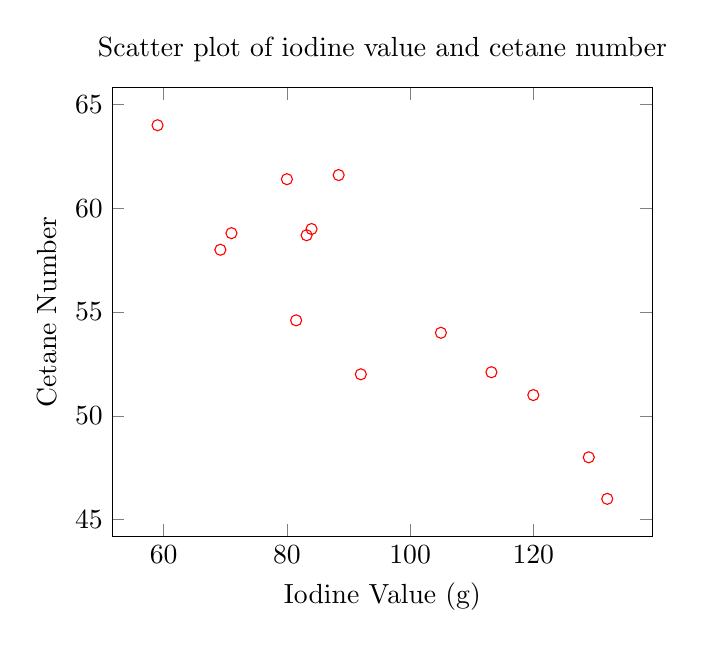
\begin{tikzpicture}
\begin{axis}[%
    title={Scatter plot of iodine value and cetane number},
    xlabel={Iodine Value (g)},
    ylabel={Cetane Number},
    scatter/classes={%
    a={mark=o,draw=red}}]
    \addplot[scatter,only marks,%
    scatter src=explicit symbolic]%
table[meta=label] {
x y label
132.0 46.0 a
129.0 48.0 a
120.0 51.0 a
113.2 52.1 a
105.0 54.0 a
92.0 52.0 a
84.0 59.0 a
83.2 58.7 a
88.4 61.6 a
59.0 64.0 a
80.0 61.4 a
81.5 54.6 a
71.0 58.8 a
69.2 58.0 a
};
\end{axis}
\end{tikzpicture}
    \caption{The scatter plot of iodine value (x) and cetane number (y).}
\end{figure}

Under the additional assumption that $\varepsilon_i$'s are iid $N(0, \sigma^2)$, the likelihood function of the sample is
\begin{align*}
    L(\alpha, \beta, \sigma^2 | \mathbf{y}, \mathbf{x}) = \prod_{i=1}^n f_Y(y_i | x_i, \alpha, \beta, \sigma^2) &= \prod_{i=1}^n \frac{1}{\sqrt{2\pi\sigma^2}} \exp\left(-\frac{(y_i - \alpha - \beta x_i)^2}{2\sigma^2}\right)\\
    &= \frac{1}{(2\pi\sigma^2)^{n/2}} \exp\left(-\frac{1}{2\sigma^2} \sum_{i=1}^n (y_i - \alpha - \beta x_i)^2\right). \label{eq:s2.1} \tag{{\color{gray} $\spadesuit $}} 
\end{align*}

Considering $(y_1, x_1), \ldots, (y_n, x_n)$ as $n$ pairs of data points plotted 
in the $xy$-plane as the scatterplot in the previous figure.

Think of drawing through this cloud of points a straight line that comes
``as close as possible`` to all the points, measured by the vertical
 distances from the points to the straight line. For any line 
$y = \alpha + \beta x$, the vertical distance from the point $(x_i, y_i)$ to the line is $y_i - (\alpha + \beta x_i)$.
Letting
\[
    \psi(\alpha, \beta) := \sum_{i=1}^n (y_i - \alpha - \beta x_i)^2,
\]

Maximizing the likelihood is equivalent to
\[
    \min_{\alpha, \beta} \sum_{i=1}^n (y_i - \alpha - \beta x_i)^2,
\]

Taking the partial derivatives of $\psi(\alpha, \beta)$ with respect to $\alpha$ and $\beta$, we have
\[
    \pdv{\psi(\alpha, \beta)}{\alpha} = -2 \sum_{i=1}^n (y_i - \alpha - \beta x_i) = 0,
\]
\[
    \pdv{\psi(\alpha, \beta)}{\beta} = -2 \sum_{i=1}^n x_i (y_i - \alpha - \beta x_i) = 0. \label{eq:s2.0} \tag{{\color{orange!50!white} $\clubsuit $}}
\]
The first equation gives
\[
    \overline{y} - a -b\overline{x} \implies a = \overline{y} - b\overline{x}.
\]
Substituting $a$ into the second equation \eqref{eq:s2.0} by $\overline{y} - b\overline{x}$ results in
\[
    \sum_{i=1}^n x_i (y_i - \overline{y}) + b \sum_{i=1}^n x_i (\overline{x} - x_i) = 0.
\]
This equation is the same as $S_{xy} = b S_{xx}$, that is
\[
    S_{xy} = \sum_{i=1}^n (x_i - \overline{x})(y_i - \overline{y}), \quad S_{xx} = \sum_{i=1}^n (x_i - \overline{x})^2.
\]
Therefore, replacing $y_i$ by the random variable $Y_i$ for all $i = 1, 2, \ldots, n$ (and we 
still use $S_{xy}$ when $y_i$ is replaced by $Y_i$), we obtain the MLE or LSE as 
\begin{equation}
    \widehat{\beta} = \frac{S_{xy}}{S_{xx}}, \quad \widehat{\alpha} = \overline{Y} - \widehat{\beta} \overline{x} = \overline{Y} - \frac{S_{xy}}{S_{xx}} \overline{x}.
\end{equation}
We can always assume that $S_{xx} > 0$, since $S_{xx} = 0$ is the trivial case of identical $x_i$'s.

We now proceed to show that $\widehat{\alpha}$ and $\widehat{\beta}$ are UMVUE of $\alpha$ and $\beta$, respectively. First of all, 
we had already shown that they are unbiased estimators of $\alpha$ and $\beta$, respectively.
\[
    \mathbb{E}[S_{xy}] = \sum^n_{i=1} (x_i - \overline{x}) \mathbb{E}_y(y_i - \overline{y}) = \sum^n_{i=1} (x_i - \overline{x}) \beta (x_i - \overline{x}) =  \beta S_{xx}.
\]
Since $\widehat{\beta}$ is unbiased for $\beta$ and 
\[
    \mathbb{E}[\widehat{\alpha}] = \mathbb{E}[\overline{Y}] - \overline{x} \mathbb{E}[\widehat{\beta}] = \alpha + \beta \overline{x} - \overline{x} \beta = \alpha.
\]
Continue with \eqref{eq:s2.1}, the likelihood function of the sample is
\begin{align*}
    L(\alpha, \beta, \sigma^2 | \mathbf{y}, \mathbf{x}) &= \frac{1}{(2\pi\sigma^2)^{n/2}} \exp\left(-\frac{1}{2\sigma^2} \sum_{i=1}^n (y_i - \alpha - \beta x_i)^2\right)\\
    &= \frac{1}{(2\pi\sigma^2)^{n/2}} \exp\left(-\frac{1}{2\sigma^2} \left[ \sum_{i=1}^n (y_i - \overline{y})^2 + n(\overline{y} - \alpha - \beta \overline{x})^2 + (\beta - \widehat{\beta})^2 S_{xx} \right] \right).
\end{align*}

where 
\[
    S_{yy} = \sum_{i=1}^n (y_i - \overline{y})^2.
\]
We still using the notation $S_{xy}$ and $S_{xx}$ when $y_i$ is replaced by $Y_i$. From the properties of the exponential family, a complete and sufficient
statistic for $\underline{\theta} = (\alpha, \beta, \sigma^2)$ is given by $(\widehat{\alpha}, \widehat{\beta}, S_{yy})$.

Since $\widehat{\alpha}$ and $\widehat{\beta}$ are both unbiased estimators and functions of the sufficient and complete 
statistic, thus they are UMVUE of $\alpha$ and $\beta$, respectively.

\end{example}
\begin{example}[Simple linear regression (cont.)]
    \textbf{Question: What if we remove the normality assumption? } 
    $\widehat{\alpha}$ and $\widehat{\beta}$ are still least squares estimators, but they are no longer MLEs.
    A statistical property that holds for LSE is that it is the best linear unbiased estimator (BLUE) 
    in the sense that $\widehat{\alpha}$ or $\widehat{\beta}$ has the smallest variance among all linear unbiased estimators of the form 
    \begin{equation}
        \sum^n_{i=1} d_i Y_i
    \end{equation}

If the estimator of this form is unbiased for $\beta$, then 
\begin{align*}
    \beta = \mathbb{E}_y\left( \sum^n_{i=1} d_iY_i \right) &= \sum^n_{i = 1} d_i \mathbb{E}_y[Y_i]\\
    &= \sum^n_{i = 1} d_i (\alpha + \beta x_i) & \text{from the regression line, } \widehat{Y} = \alpha + \beta x\\
    &= \alpha \sum^n_{i = 1} d_i + \beta \sum^n_{i = 1} d_i x_i & \text{linearity of summation}.
\end{align*}

holds for all $\alpha$ and $\beta$, which imples that 
\[
    \sum^n_{i = 1} d_i = 0, \quad \sum^n_{i = 1} d_i x_i = 1.
\]
A geometric description  of the BLUE of $\beta$ is given in the filgure below.

% TODO: Computation of 3d graph requires longer time, this should left 
% for last part
\begin{comment}
    \begin{figure}[ht]
        \centering
        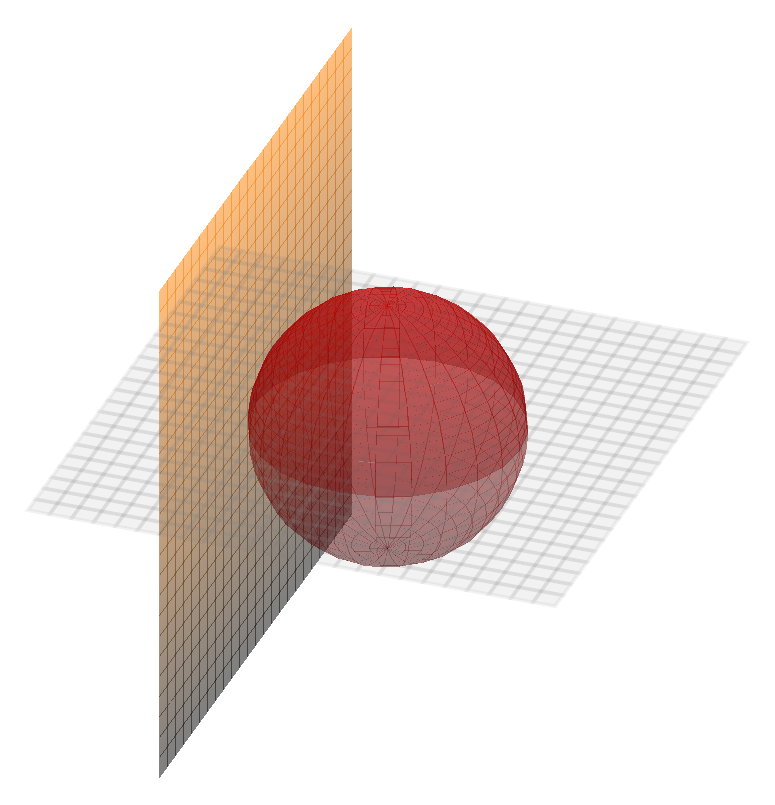
\begin{tikzpicture}[scale=3.25]
    \begin{axis}
    [   axis equal,
        hide axis,
        view={20}{30},
        z buffer=sort,
    ]
        \addplot3
        [   domain=-2:2,
            y domain=-2:2,
            surf,
            mesh/interior colormap=
           {blueblack}{color=(black) color=(orange)},
            mesh/interior colormap thresh=1,
            shader=interp,
            opacity=0.5,
        ] (-1,y,x);
        \addplot3
        [   domain=0:360,
            y domain=0:180,
            surf,
            mesh/interior colormap=
           {blueblack}{color=(black) color=(red)},
            mesh/interior colormap thresh=1,
            shader=interp,
            opacity=0.3
        ] ({sin(y)*cos(x)},{sin(y)*sin(x)},{cos(y)});
        \addplot3
        [   domain=-2:2,
            y domain=-2:2,
            surf,
            shader=flat,
            gray,
            opacity=0.1,
        ] (x,y,0);
        \addplot3
        [   domain=0:360,
            y domain=0:90,
            surf,
            mesh/interior colormap=
           {blueblack}{color=(black) color=(red)},
            mesh/interior colormap thresh=1,
            shader=interp,
            opacity=0.3,
        ] ({sin(y)*cos(x)},{sin(y)*sin(x)},{cos(y)});
    \end{axis}
\end{tikzpicture}
    \end{figure}
\end{comment}

We want to show the LSE $\widehat{\beta}$ is BLUE. Since 
\[
    Var \left( \sum^n_{i=1} d_i Y_i \right) = \sigma^2 \sum^n_{i=1} d^2_i,
\]
the BLUE of $\beta$ is the solution of the optimization problem
\begin{subequations}
\begin{alignat}{2}
&\!\min_{d_i}        &\qquad& \sum_{i=1}^{n} d^2_i\\
&\text{subject to} &      & \sum^n_{i = 1} d_i = 0,\\
&                  &      & \sum^n_{i = 1} d_i x_i = 1.
\end{alignat}
\end{subequations}

Consider the Lagrange multiplier method by minimizing 
\begin{equation}
    g(d_1, \ldots, d_n, \lambda_1, \lambda_2) = \sum_{i=1}^{n} d^2_i + \lambda_1 \left( \sum^n_{i = 1} d_i \right) + \lambda_2 \left( \sum^n_{i = 1} d_i x_i - 1 \right).
\end{equation}

Taking derivatives with respect to $d_i$ and setting them to zero, we have
\[
    \pdv{g}{d_i} = 2d_i + \lambda_1 + \lambda_2 x_i = 0.
\]
Then
\begin{align*}
    0 = \sum_{i=1}^{n} (2d_i + \lambda_1 + \lambda_2 x_i) &= 2 \sum_{i=1}^{n} d_i + n\lambda_1 + \lambda_2 \sum_{i=1}^{n} x_i & \text{linearity of summation}\\
    &= \lambda_1 n + \lambda_2 \sum^n_{i=1} x_i & \text{since } \sum d_i = 0
\end{align*}
which yields $\lambda_1 = - \lambda_2 \overline{x}$ and, hence
\[
    0 = 2d_i + \lambda_2 (x_i - \overline{x}).
\]
Then 
\[
    0 = \sum^n_{i=1} (x_i - \overline{x}) [2d_i + \lambda_2 (x - \overline{x})] = 2 + \lambda_2 S_{xx}
\]
which gives us $\lambda_2 = -2 / S_{xx}$. Then 
\[
    d_i = \frac{-(\lambda_1 + \lambda_2 x_i)}{2} = \frac{-\lambda_2(x_i - \overline{x})}{2}
    = \frac{(x_i - \overline{x})}{S_{xx}}
\]
and the BLUE of $\beta$ is 
\[
    \sum^n_{i=1} d_i Y_i = \sum_{i=1}^{n} \frac{(x_i - \overline{x})}{S_{xx}} Y_i = \frac{S_{xy}}{S_{xx}} = \widehat{\beta}.
\]
And because
\[
    \widehat{\beta} = \sum_{i=1}^{n} \frac{(x_i - \overline{x})(\beta x_i + \varepsilon_i)}{S_{xx}}
    = \beta + \sum^n_{i=1} d_i \varepsilon_i
\]
where $d_i = (x_i - \overline{x})/S_{xx}$, and the random error $\varepsilon \sim N(0,1)$. We obtain that 
\[
    Var(\widehat{\beta}) = \sum_{i=1}^{n} d^2_i Var(\varepsilon_i) = \frac{\sigma^2}{S_{xx}}.
\]
And we are done.
\end{example}


\begin{corollary}[Cramér-Rao lower bound - 2nd theorem]
    If $L(\theta)$ is twice differentiable with respect to $\theta$, then the inequality 
    can be stated equivalently as
    \begin{equation}
        \text{Var}(\widehat{\theta}) \geq \frac{-1}{\mathbb{E} \left[ \pdv[order={2}]{\ln L(\theta)}{\theta} \right]}.
    \end{equation}
\end{corollary}
\begin{proof}
    If $L(\theta)$ is twice differentiable, then $\pdv[order={2}]{\ln L(\theta)}{\theta}$ exists. 
    And since that $L(\theta)$ is maximum likelihood so we have
    \[
        \pdv[order={2}]{\ln L(\theta)}{\theta} < 0.
    \]
    Hence the sign of the right-hand side of the Cramér-Rao inequality must be negative.
\end{proof}

\begin{example}
    Let $X_1, X_2, \ldots, X_n$ be a random samples from a distribution with density function
    \[
        f(x|\theta) = \begin{cases}
            3\theta x^2 e^{-\theta x^3} & \text{if } 0 < x < \infty\\
            0 & \text{otherwise}.
        \end{cases}
    \]
    What is the Cramér-Rao lower bound for the variance of unbiased estimator of the parameter $\theta$?
\end{example}
\begin{solution}
    Let $\widehat{\theta}$ be an unbiased estimator of $\theta$. Cramér-Rao lower bound for 
    the variance of $\widehat{\theta}$ is given by
    \[
        \text{Var}(\widehat{\theta}) \geq \frac{-1}{\mathbb{E} \left[ \left( \odv{\ln L(\theta)}{\theta} \right)^2 \right]}.
    \]
    First, compute the likelihood function for the sample:
    \[
        L(\theta) = \prod_{i=1}^n f(x_i|\theta) = \prod_{i=1}^n 3\theta x_i^2 e^{-\theta x_i^3} = 3^n \theta^n \left(\prod_{i=1}^n x_i^2\right) \exp\left(-\theta \sum_{i=1}^n x_i^3\right).
    \]
    Take the log-likelihood:
    \[
        \ell(\theta) = \ln L(\theta) = n\ln 3 + n\ln \theta + 2\sum_{i=1}^n \ln x_i - \theta \sum_{i=1}^n x_i^3.
    \]
    Compute the first derivative with respect to $\theta$:
    \[
        \frac{\partial}{\partial \theta} \ell(\theta) = \frac{n}{\theta} - \sum_{i=1}^n x_i^3.
    \]
    Compute the second derivative:
    \[
        \frac{\partial^2}{\partial \theta^2} \ell(\theta) = -\frac{n}{\theta^2}.
    \]
    The Fisher information for one observation is
    \[
        I_X(\theta) = -\mathbb{E}\left[\frac{\partial^2}{\partial \theta^2} \ln f(X|\theta)\right] = \frac{1}{\theta^2}.
    \]
    For $n$ independent observations, the total Fisher information is $n I_X(\theta) = \frac{n}{\theta^2}$.

    Therefore, the Cramér-Rao lower bound is
    \[
        \text{Var}(\widehat{\theta}) \geq \frac{1}{n I_X(\theta)} = \frac{\theta^2}{n}.
    \]
    where $L(\theta)$ denotes the likelihood function of the given random sample.
\end{solution}

\begin{example}
    Let $X_1, X_2, \ldots, X_n$ denote a random sample from $Bin(1, p)$. We knew that $\ols{X}$ is an 
    unbiased estimator of $p$ and that 
    \[
        Var(\ols{X}) = \frac{p(1-p)}{n}.
    \]
    Find the Cramér-Rao lower bound for the variance of every unbiased estimator of $p$.
\end{example}
\begin{solution}
    This is a Bernoulli distribution with parameter $p$. The denisty function for each $X_i$ is 
    \[
        f(x|p) = p^x (1-p)^{1-x}, \quad x = 0,1.
    \]
    Taking logarithm on $f$,
    \[
        \ln f(x|p) = \ln p^x + \ln (1-p)^{1-x} = \fbox{$x \ln p + (1-x) \ln (1-p)$} \label{eq:s1.5} \tag{{\color{Red} $\blacklozenge $}}
    \]
    Compute the first and second order derivative of \eqref{eq:s1.5} with respect to $p$. The second 
    order derivative will be the Fisher information. In this case we have only one parameter which is $p$, so the information 
    is just a simple algebraic expression rather than a matrix.
    \[
        \frac{\partial \ln f(x|p)}{\partial p} = \frac{x}{p} + \frac{x-1}{1-p}
    \]
    \begin{align*}
        \frac{\partial^2 \ln f(x|p)}{\partial p^2} &= -\frac{x}{p^2} + (-1)^2(x-1)(1-p)^{-2}\\
        &= -\frac{x}{p^2} + \frac{x-1}{(1-p)^2}. \label{eq:s1.6} \tag{{\color{YellowOrange} $\blacktriangle$}}
    \end{align*}
    Hence we find the expectation of $x$ in \eqref{eq:s1.6}, that is
    \begin{align*}
        \mathbb{E}_X \left[ \frac{\partial^2 \ln f(x|p)}{\partial p^2} \right] &= \mathbb{E}_X \left[ -\frac{x}{p^2} + \frac{x-1}{(1-p)^2} \right]\\
        &= - \frac{1}{p^2} \mathbb{E}_X[X] + \frac{1}{(1 - p)^2} \mathbb{E}_X[X - 1]\\
        &= - \frac{p}{p^2} + \frac{p-1}{(1 - p)^2}\\
        &= - \frac{1}{p(1-p)}.
    \end{align*}
    Therefore, the Cramér-Rao lower bound for the variance of unbiased estimator of $p$ is 
    \[
        Var(\widehat{p}) \geq - \frac{1}{-n I_X(p)} = \frac{1}{\displaystyle \frac{-n}{-p(1-p)}} = \frac{p(1-p)}{n}.
    \]
\end{solution}

\subsection{Delta method -- Variance of functions of estimators}

The Delta Method (DM) states that we can approximate the asymptotic behaviour of functions over a random variable, if the random variable is itself asymptotically normal. In practice, this theorem tells us that even if we do not know the expected value and variance of the function  
$g(X)$ we can still approximate it reasonably. Note that by Central Limit Theorem we know that several important random variables and estimators are asymptotically normal, including the sample mean. We can therefore approximate the mean and variance of some transformation of the sample mean using its variance.

More specifically, suppose that we have some sequence of random variables $\{X_n\}$, as $n \to \infty$,

Given this, if $g$ is some smooth function (i.e. there are no discontinuous jumps in values) then the Delta Method states that:
\begin{equation}
    \frac{\sqrt{n} (g(X_n) - g(\mu))}{|\dot{g}(\mu)|\sigma} \approx \mathcal{N}(0,1)
\end{equation}

DM also generalizes to multidimensional functions, where instead of converging on the standard normal the random variable must converge in distribution to a multivariate normal, and the derivatives of  
$g$ are replaced with the gradient of g (a vector of all partial derivatives).

\begin{theorem}[Delta method]
    Suppose that $g(\theta)$ is a function of estimator.
    The delta method provides a way to approximate the variance of a function of an estimator.
    This approximate of the variance is given by
    \begin{equation}
        Var(g(\widehat{\theta})) \approx [\dot{g}(\theta)]^2\, Var[\widehat{\theta}].
    \end{equation}
\end{theorem}

\begin{example}
    Given $g(s,t) = \mfrac{s}{t}$, $h(s,t) = \ln s$ and 
    $\widehat{\theta}_1$ and $\widehat{\theta}_2$ are unbiased estimators of $\theta_1$ and $\theta_2$. Based 
    on a particular sample, the maximum likelihood estimates of $\theta_1$ and $\theta_2$ are $\widehat{\theta}_1 = 3.2$ and $\widehat{\theta}_2 = 11.8$, 
    and the log-likelihood is $\ell(\theta_1, \theta_2) = -2\theta_1^2 \theta_2 - \theta_2^3$.
\end{example}
\begin{solution}
    We first compute the Fisher information matrix:
    \[
        \frac{\partial^2}{\partial \theta_1^2} \ell(\theta_1, \theta_2) = -4\theta_2, \quad
        \frac{\partial^2}{\partial \theta_2^2} \ell(\theta_1, \theta_2) = -6\theta_2, \quad
        \frac{\partial^2}{\partial \theta_1 \partial \theta_2} \ell(\theta_1, \theta_2) = -4\theta_1.
    \]
    The information matrix is 
    \[
        I_X(\theta) = -\mathbb{E} \begin{bmatrix}
            \frac{\partial^2}{\partial \theta_1^2} \ell(\theta_1, \theta_2) & \frac{\partial^2}{\partial \theta_1 \partial \theta_2} \ell(\theta_1, \theta_2) \\
            \frac{\partial^2}{\partial \theta_1 \partial \theta_2} \ell(\theta_1, \theta_2) & \frac{\partial^2}{\partial \theta_2^2} \ell(\theta_1, \theta_2)
        \end{bmatrix} = \begin{bmatrix}
            4\theta_2 & 4\theta_1 \\
            4\theta_1 & 6\theta_2
        \end{bmatrix}.
    \]
    The covariance matrix of the MLEs is given by the inverse of the Fisher information matrix evaluated at the MLEs:
    \[
        \Sigma = I_X(\theta)^{-1} = \begin{bmatrix}
            4\theta_2 & 4 \theta_1 \\
            4\theta_1 & 6 \theta_2
        \end{bmatrix}^{-1} = \frac{1}{12 \theta_2^2 - 8\theta^2_1} \begin{bmatrix}
            3\theta_2 & -2\theta_1 \\
            -2\theta_1 & 2\theta_2
        \end{bmatrix}.
    \]
    The estimated covariance matrix is obtained by substituting the MLEs:
    \begin{align*}
        \widehat{\Sigma} 
        = \frac{1}{12 \widehat{\theta}_2^2 - 8\widehat{\theta}^2_1} \begin{bmatrix}
            3\widehat{\theta}_2 & -2\widehat{\theta}_1 \\
            -2\widehat{\theta}_1 & 2\widehat{\theta}_2
        \end{bmatrix}
        &= \frac{1}{12(11.8)^2 - 8(3.2)^2} \begin{bmatrix}
            3(11.8) & -2(3.2) \\
            -2(3.2) & 2(11.8)
        \end{bmatrix}\\ 
        &= \begin{bmatrix}
            0.0222787 & -0.00402779 \\
            -0.00402779 & 0.0148525
        \end{bmatrix}\\[0.6em]
        &= \begin{bmatrix}
            Var(\widehat{\theta}_1) & \cov(\widehat{\theta}_1, \widehat{\theta}_2)\\
            \cov(\widehat{\theta}_1, \widehat{\theta}_2) & Var(\widehat{\theta}_2)
        \end{bmatrix}.
    \end{align*}

    \begin{enumerate}
        \item Now take partial derivatives of $g(s,t)$ with respect to $s$ and $t$:
        \[
            g_s(s,t) = \frac{\partial g}{\partial s} = \frac{1}{t} \Longrightarrow g_s(\widehat{\theta}_1, \widehat{\theta}_2) = \frac{1}{11.8},
        \]
        \[
            g_t(s,t) = \frac{\partial g}{\partial t} = -\frac{s}{t^2} \Longrightarrow g_t(\widehat{\theta}_1, \widehat{\theta}_2) = -\frac{3.2}{(11.8)^2}.
        \]
        Hence, 
        let $\mathbf{w} = \begin{bmatrix}
            g_s(\widehat{\theta}_1, \widehat{\theta}_2) &
            g_t(\widehat{\theta}_1, \widehat{\theta}_2)
        \end{bmatrix} = \begin{bmatrix}
            \mfrac{1}{11.8} &
            -\mfrac{3.2}{11.8^2}
        \end{bmatrix}$.
        the approximate variance of $g(\widehat{\theta}_1, \widehat{\theta}_2)$ is
        \begin{align*}
            Var(g(\widehat{\theta}_1, \widehat{\theta}_2)) &\approx \mathbf{w} \widehat{\Sigma} \mathbf{w}^T \\
            &= \begin{bmatrix}
                \mfrac{1}{11.8} &
                -\mfrac{3.2}{11.8^2}
            \end{bmatrix}
            \begin{bmatrix}
                0.0222787 & -0.00402779 \\
                -0.00402779 & 0.0148525
            \end{bmatrix}
            \begin{bmatrix}
                \mfrac{1}{11.8} \\[0.6em]
                -\mfrac{3.2}{11.8^2}
            \end{bmatrix}\\[0.6em]
            &= 0.000208785.
        \end{align*}

        \item Continue with $h(s,t)$: take partial derivatives of $h(s,t)$ with respect to $s$ and $t$:
        \[
            h_s(s,t) = \frac{\partial h}{\partial s} = \frac{1}{s} \Longrightarrow h_s(\widehat{\theta}_1, \widehat{\theta}_2) = \frac{1}{3.2},
        \]
        \[
            h_t(s,t) = \frac{\partial h}{\partial t} = 0 \Longrightarrow h_t(\widehat{\theta}_1, \widehat{\theta}_2) = 0.
        \]
        The estimated covariance between $h(\widehat{\theta}_1, \widehat{\theta}_2)$ and $g(\widehat{\theta}_1, \widehat{\theta}_2)$ is
        \begin{align*}
            \cov(h(\widehat{\theta}_1, \widehat{\theta}_2), g(\widehat{\theta}_1, \widehat{\theta}_2)) &=
            \begin{bmatrix}
                \mfrac{1}{\widehat{\theta}_1} &
                -\mfrac{\widehat{\theta}_1}{\widehat{\theta}_2^2}
            \end{bmatrix}
            \begin{bmatrix}
                0.0222787 & -0.00402779 \\
                -0.00402779 & 0.0148525
            \end{bmatrix}
            \begin{bmatrix}
                \mfrac{1}{\widehat{\theta}_1} \\[0.6em]
                0
            \end{bmatrix}\\[0.6em]
            &= \begin{bmatrix}
                \mfrac{1}{11.8} &
                -\mfrac{3.2}{11.8^2}
            \end{bmatrix}
            \begin{bmatrix}
                0.0222787 & -0.00402779 \\
                -0.00402779 & 0.0148525
            \end{bmatrix}
            \begin{bmatrix}
                \mfrac{1}{3.2} \\[0.6em]
                0
            \end{bmatrix}\\[0.6em]
            &= 6.2 \times 10^{-3}
        \end{align*}
    \end{enumerate}
\end{solution}

\section*{Tutorials}

\begin{mdframed}
    \vspace{-0.25cm}
    \hspace{-0.25cm}
    \begin{Exercise}
        If $X$ is uniformly distributed on the interval $(2\theta, 3\theta)$ where $\theta > 0$. 
        And that $X_1, X_2, \ldots, X_n$ is a random sample from the distribution of $X$.
        Find the bias in the maximum likelihood estimator of $\theta$.
    \end{Exercise}

    \begin{Exercise}
        Let $X_1, X_2, \ldots, X_n$ be a random sample from a population 
        $X \sim Poisson(\lambda)$, where $\lambda > 0$ is a parameter. Is the 
        estimator $\ols{X}$ of $\lambda$ a consistent estimator of $\lambda$?
    \end{Exercise}

    \begin{Exercise}
        Let $X_1, X_2, \ldots, X_n$ be a random sample from a population 
        $X$ with density function 
        \[
            f(x|\theta) = \begin{cases}
                \theta x^{\theta - 1} & \text{for } 0 < x < 1\\
                0 & \text{otherwise},
            \end{cases}
        \]
        where $\theta > 1$ is a parameter. Show that 
        \[
            -\frac{1}{n} \sum_{i=1}^{n} \ln(X_i) 
        \]
        is a uniform minimum variance unbiased estimator of $\mfrac{1}{\theta}$.
    \end{Exercise}

    \begin{Exercise}
        Let $Y_1, Y_2, \ldots, Y_n$ denote a random sample from a population with mean $\mu$ and 
        variance $\sigma^2$. Consider the following three estimators for $\mu$:
        \[
            \widehat{\mu}_1 = \frac{1}{2}(Y_1 + Y_2), \quad 
            \widehat{\mu}_2 = \frac{1}{4}Y_1 + \frac{Y_2 + \ldots + Y_{n-1}}{2(n-2)} + \frac{1}{4}Y_n, \quad 
            \widehat{\mu}_3 = \ols{Y}.
        \]
        \begin{enumerate}
            \item Show that each of the three estimators is unbiased.
            \item Find the efficiency of $\widehat{\mu}_3$ relative to $\widehat{\mu}_2$ and $\widehat{\mu}_1$, respectively.
        \end{enumerate}
    \end{Exercise}

    \begin{Exercise}
        \begin{enumerate}
            \item State the definition of unbiased estimator.
            \item Show that if $\widehat{\Theta}_1$ is an unbiased estimator for $\theta$, and $W$ is a zero mean random variable, then 
            \[
                \widehat{\Theta}_2 = \widehat{\Theta}_1 + W
            \]
            is also an unbiased estimator for $\theta$.
            \item Show that if $\widehat{\Theta}_1$ is an unbiased estimator for $\theta$ such that $\mathbb{E}[\widehat{\Theta}_1] = a\theta + b$, where $a \neq 0$. Then 
            \[
                \widehat{\Theta}_2 = \frac{\widehat{\Theta}_1 - b}{a}
            \]
            is an unbiased estimator for $\theta$.
        \end{enumerate}
    \end{Exercise}

    \begin{Exercise}
        Given $\theta = \begin{bmatrix}
            \theta_1 \\ \theta_2
        \end{bmatrix}$
        is a vector of parameters being estimated by maximum likelihood. You are 
        given that the current value of the vector of estimates is 
        $\widehat{\theta} = \begin{bmatrix}
            30 \\ 2
        \end{bmatrix}$ as well as the estimated information matrix 
        \[
            I(\widehat{\theta}) = \begin{bmatrix}
                .075 & -.620\\
                -.620 & 10.0
            \end{bmatrix}.
        \]
        Determine the approximate variance of $\widehat{\theta}_1$.
    \end{Exercise}

    \begin{Exercise}
        Let $X$ be a random variable, and $X_n = X + Y_n$, where 
        \[
            \mathbb{E}[Y_n] = \frac{1}{n} \quad \text{ and } \quad Var(Y_n) = \frac{\sigma^2}{n}.
        \]
        where $\sigma > 0$ is constant. Show that $X_n \xrightarrow{p} X$ as $n \to \infty$. Hint: $\displaystyle |Y_n| \leq |Y_n - \mathbb{E}[Y_n]| + \frac{1}{n}$.
    \end{Exercise}
\end{mdframed}